%!TEX root = /Users/stevenmartell/Documents/CURRENT PROJECTS/iSCAM-trunk/fba/BC-herring-2011/WRITEUP/BCHerring2011.tex

\section{Stock assessments for minor stock areas}

Abundance estimates for the minor stock areas, Area 2W and Area 27 were also obtained using the \iscam\ model.  For these minor areas, there were some minor differences in the treatment of the data and model assumptions.  Also, the gillnet selectivity in area 27 was not allowed to vary over time due to the sparse amount of information (and presumably biological samples) available to reliably estimate minor changes in selectivity for this fishery. Selectivity for area 27 gillnet fishery was assumed to be a logistic function of age and invariant over time.

The input data (Catch and relative abundance) for the minor areas is shown in Figure \ref{Results:Minor:figData}.  As in the previous assessments of Area 2W, the spawn survey data is treated as a single continuous series from 1978 to 2011.  Area 27 however, the time series is split into two series between 1978-1987 and 1988-2011.  The age-composition data used in fitting the model is shown in Figure \ref{Results:Minor:figAgeComps}.




\begin{figure}[!tbp]
	% Requires \usepackage{graphicx}
	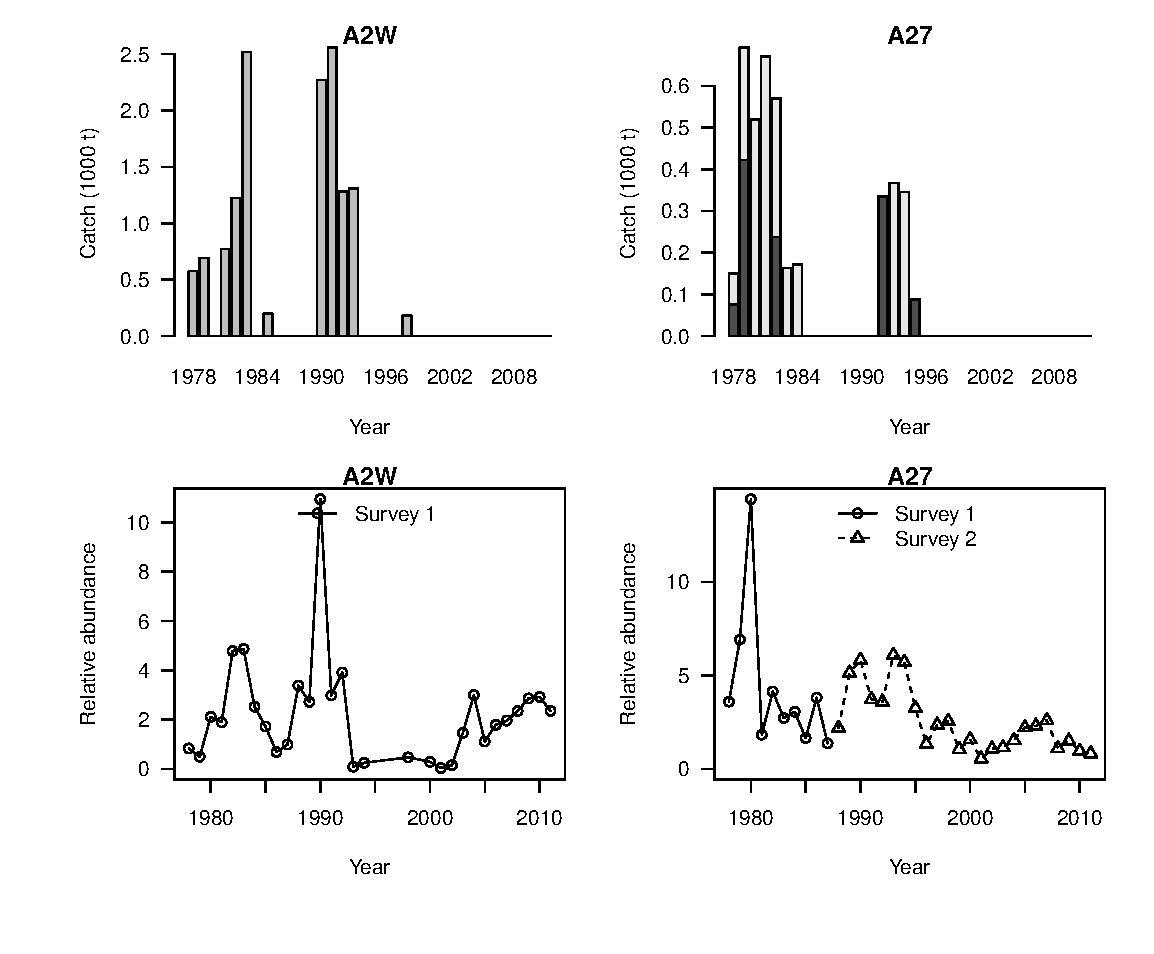
\includegraphics[width=\textwidth]{../FIGS/MinorAreas/iscam_fig_MinorAreaData.pdf}\\
	\caption{Catch and survey data for minor stock Areas 2W and Area 27.}\label{Results:Minor:figData}
\end{figure}

\begin{figure}[!tbp]
	% Requires \usepackage{graphicx}
	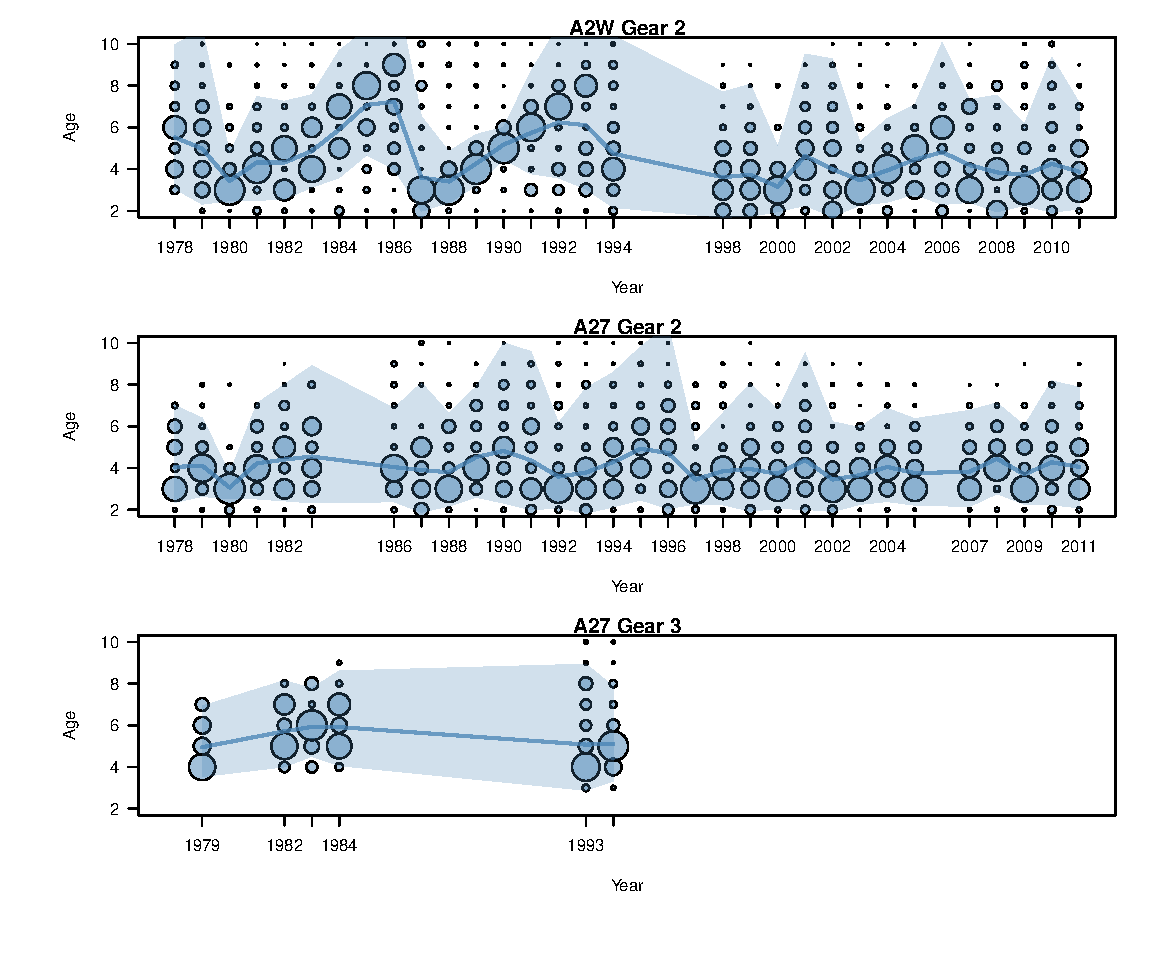
\includegraphics[width=\textwidth]{../FIGS/MinorAreas/iscam_fig_AgeCompsMinor.pdf}\\
	\caption{Age composition data for Area 2W and Area 27 for the seine-roe fishery (Gear 2) and the gillnet fishery (Gear 3).}\label{Results:Minor:figAgeComps}
\end{figure}


\subsection{Maximum likelihood estimates of biomass}

Spawning biomass in 2011 for Area 2W and Area 27 was estimated at 4,671 tonnes and 928 tonnes, respectively (Table \ref{TableRefPointsMinorAreas}).  The time series of total biomass and spawning biomass for these two areas is presented in Figure \ref{Results:Minor:figBiomass}


% latex.default(rpTable, file = fn, title = "Stock", longtable = FALSE,      landscape = FALSE, cgroup = NULL, n.cgroup = NULL, caption = cap,      label = "TableRefPoints", na.blank = TRUE, vbar = FALSE,      size = "small") 
%
\begin{table}[!tbp]
 \small
 \caption{Summary of maximum likelihood estimates for  the 
	two minor stock areas.  No. is the total number of estimated 
	parameters, \fmsy\ the average instantaneous fishing rate to 
	achieve the maximum sustainable yield (MSY), \bo\ is the unfished 
	spawning biomass, \bmsy\ is the spawning biomass that achieves 
	maximum sustainable yield,$B_t$ is the spawning biomass at the end 
	of the 2011 fishing season, and $B_t/B_0$ is the spawning depletion 
	level at the end of the 2011 fishing season.\label{TableRefPoints}} 
 \begin{center}
 \begin{tabular}{lll}\hline\hline
\multicolumn{1}{l}{Stock}&\multicolumn{1}{c}{A2W}&\multicolumn{1}{c}{A27}\tabularnewline
\hline
No.&74&79\tabularnewline
\fmsy& 0.34&  1.9\tabularnewline
MSY&  265&  304\tabularnewline
$B_0$&2,915&2,084\tabularnewline
0.25$B_0$&  729&  521\tabularnewline
\bmsy&  705&  447\tabularnewline
0.8\bmsy&  564&  358\tabularnewline
0.4\bmsy&  282&  179\tabularnewline
$B_t$&4,671&  924\tabularnewline
$B_t/B_0$&  1.6& 0.44\tabularnewline
\hline
\end{tabular}

\end{center}

\end{table}



\begin{figure}[!tbp]
	% Requires \usepackage{graphicx}
	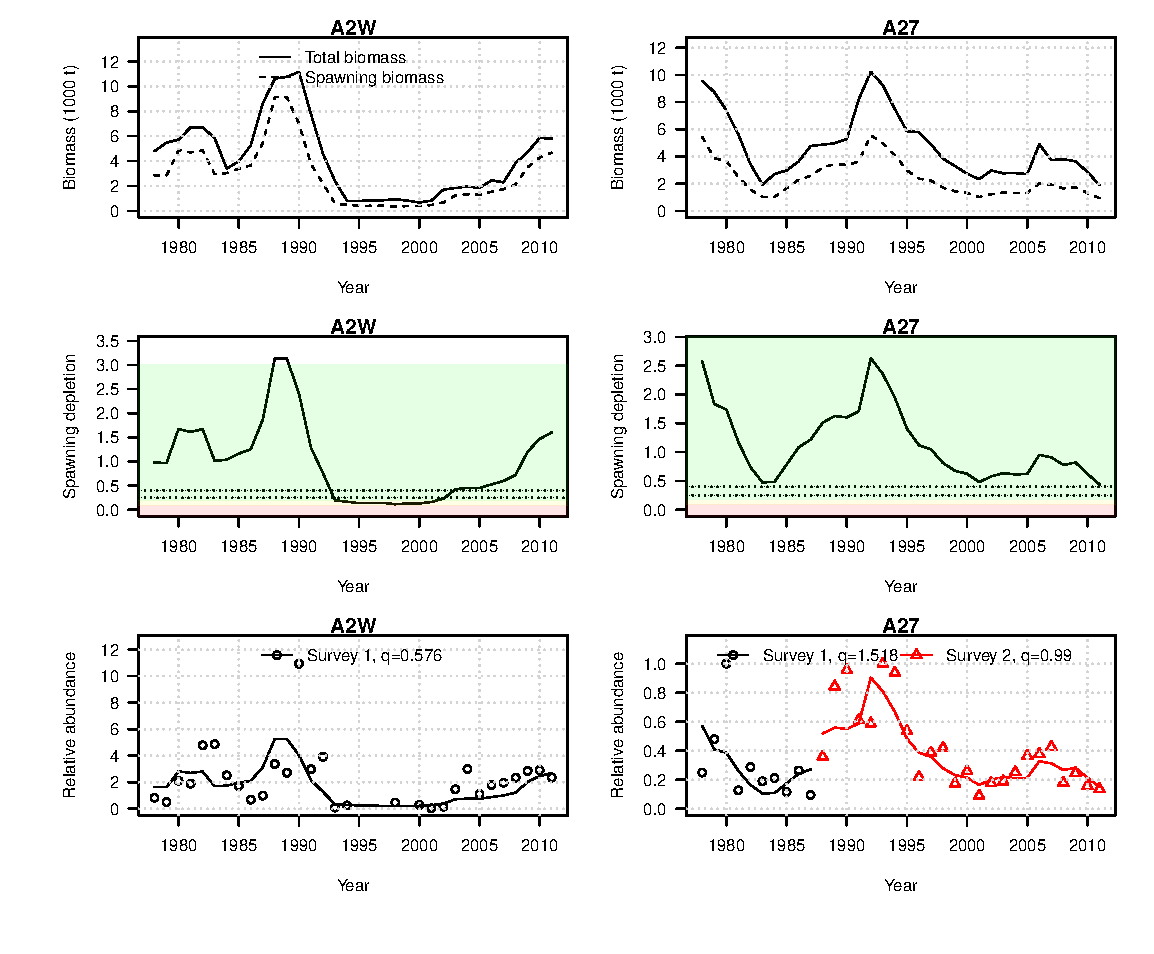
\includegraphics[width=\textwidth]{../FIGS/MinorAreas/iscam_fig_BiomassSpawnSurvey.pdf}\\
	\caption{Maximum likelihood estimates of total biomass, spawning biomass, spawning depletion and fits to the spawn survey data for the two minor stock areas.}\label{Results:Minor:figBiomass}
\end{figure}

\subsection{Estimates of recruitment and reference points}
Maximum likelihood estimates of age-2 recruitment, stock-recruitment relationships and residuals in the stock-recruitment model is shown in Figure \ref{Results:Minor:Recruitment}.  Estimates of age-2 recruits in area 2W have been poor-to average for much of the time-series.  There have been 4 periods of above average recruitment for area 2W (late 1970s, mid 1980s, 2002, and 2008-2010.  Recruitment in area 27 has been much more consistent by comparison.  Estimates of unfished spawning biomass for ares 2W and 27 are 2,915 tonnes and 2,112 tonnes.

\begin{figure}[!tbp]
	% Requires \usepackage{graphicx}
	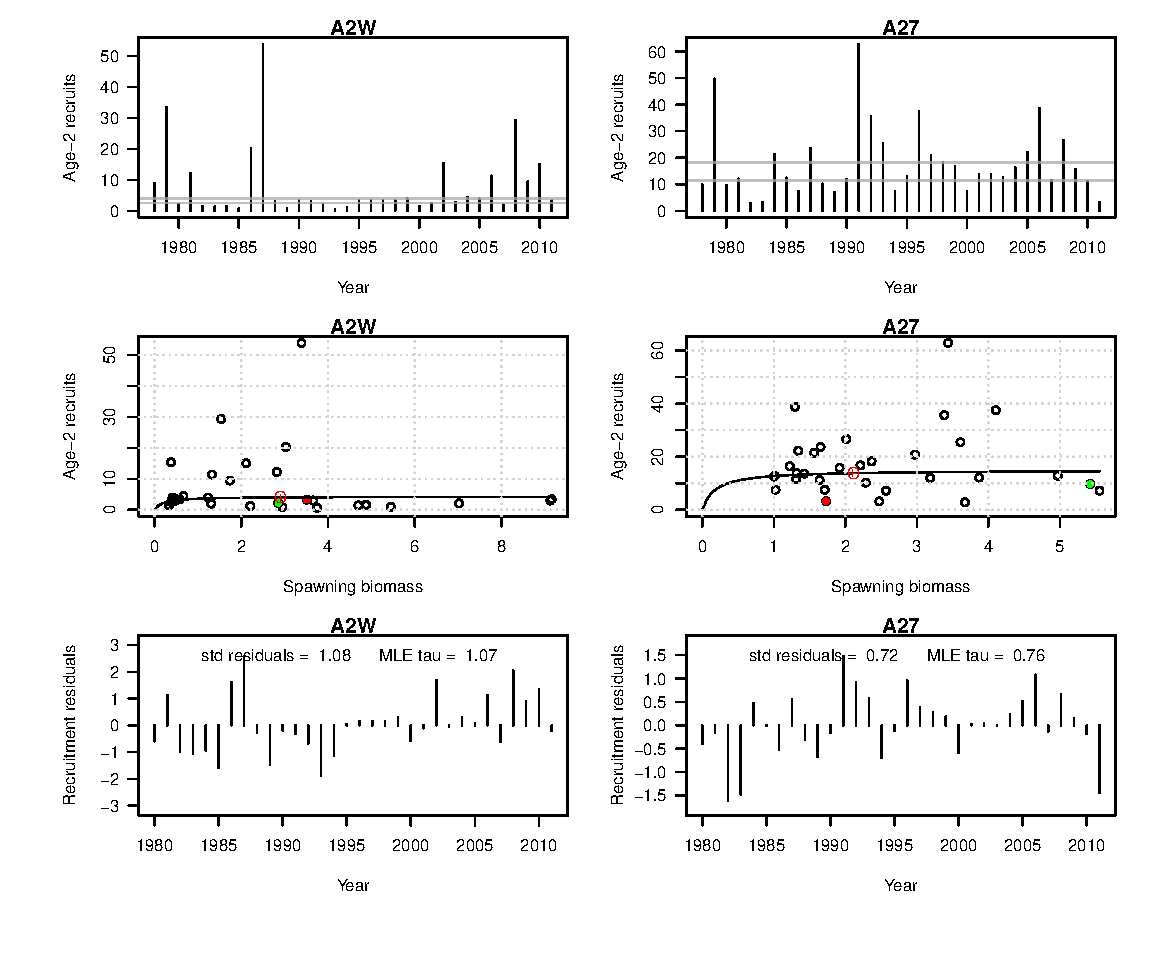
\includegraphics[width=\textwidth]{../FIGS/MinorAreas/iscam_fig_Recruitment.pdf}\\
	\caption{Maximum likelihood estimates of age-2 recruits, spawner-recruit relationships with the fitted Beverton Holt model and unfished reference points ($B_o, R_o$), and the residuals between the estimated age-2 recruits and that predicted by the Beverton-Holt model.}\label{Results:Minor:Recruitment}
\end{figure}

\subsection{Retrospective analysis}

There is almost no retrospective bias for the estimates of spawning stock biomass in area 27 using data between 1951:2001 and 1951:2011 (Fig. \ref{fig:Results:Minor:retrospective}).
In Area 2W, there is a slight retrospective bias in the estimates of spawning stock biomass.   As the more recent data are fit in the model estimates of spawning biomass in the mid 2000s are revised downwards.  In other words, there is a positive bias in estimates of spawning biomass in area 2W.

\begin{figure}[!tbp]
	% Requires \usepackage{graphicx}
	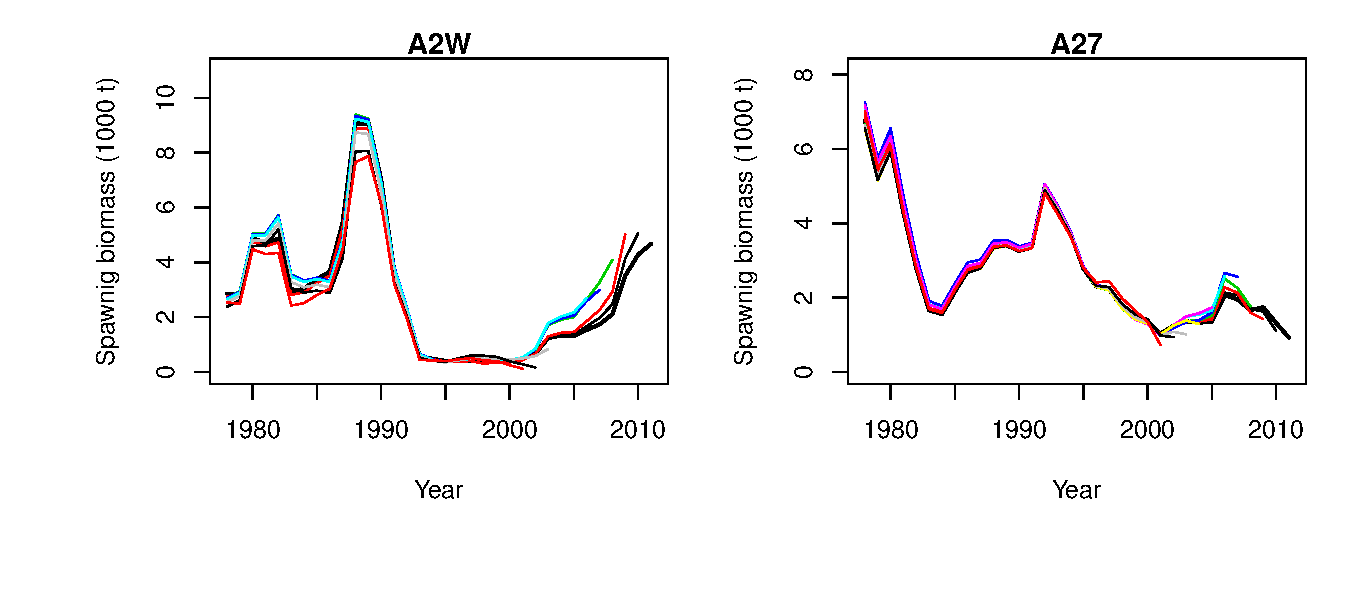
\includegraphics[width=\textwidth]{../FIGS/MinorAreas/iscam_fig_sbt_retrospective.pdf}\\
	\caption{Retrospective estimates of spawning stock biomass for each of the minor stock assessment areas.  The model was sequentially fitted to the full data set, then from 1951:2010, 1951:2009, ... 1951:2001.}\label{fig:Results:Minor:retrospective}
\end{figure}

\subsection{Marginal posterior distributions and trace plots}

Information for the catch advice for the two minor areas is based on the median values of the joint posterior distribution.  Therefore, it is important to show posterior samples to ensure proper convergence and the marginal posterior distributions for the leading parameter estimates and derived variables  that are of management interest.

 The trace plots for the two minor areas are summarized in Figure \ref{Results:Minor:mcmcTrace}, and the marginal distributions for the leading parameters is shown in Figure \ref{Results:Minor:mcmcMarginals}.  Again, no formal convergence statistics were examined to determine if MCMC chain converged to a stable distribution.  Visual inspection of the trace plots appear to have a homogenous distribution over the course of the 2000 samples.  In both of the statistical areas, the posterior updates did occur (Figure \ref{Results:Minor:mcmcMarginals}.  The marginal posterior for steepness in area 27 does appear to be influenced considerably by the assumed prior distribution.
 
 \begin{figure}[!tbp]
	% Requires \usepackage{graphicx}
	\centering
	\fbox{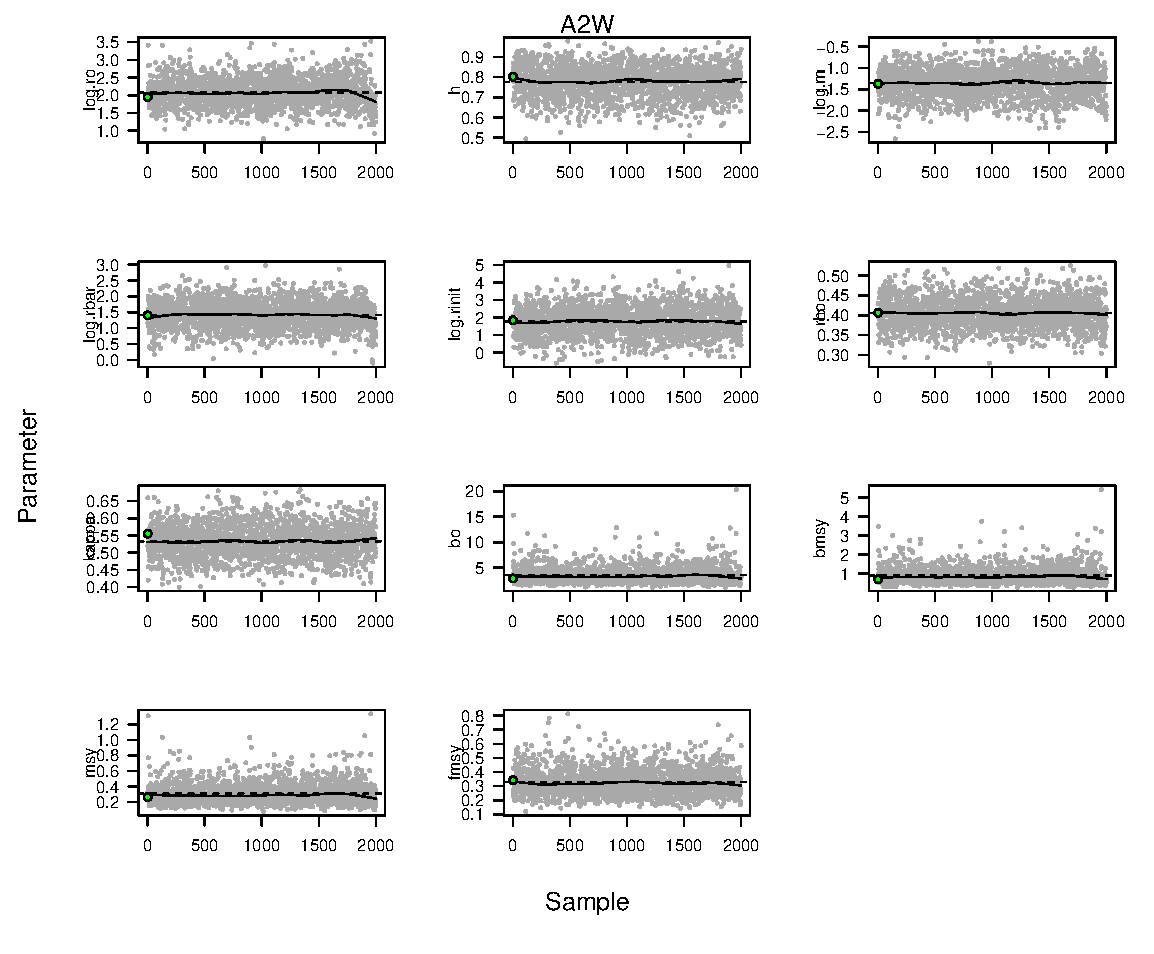
\includegraphics[width=0.75\textwidth]{../FIGS/MinorAreas/iscam_fig_traceplots_A2W.pdf}}\\
	\fbox{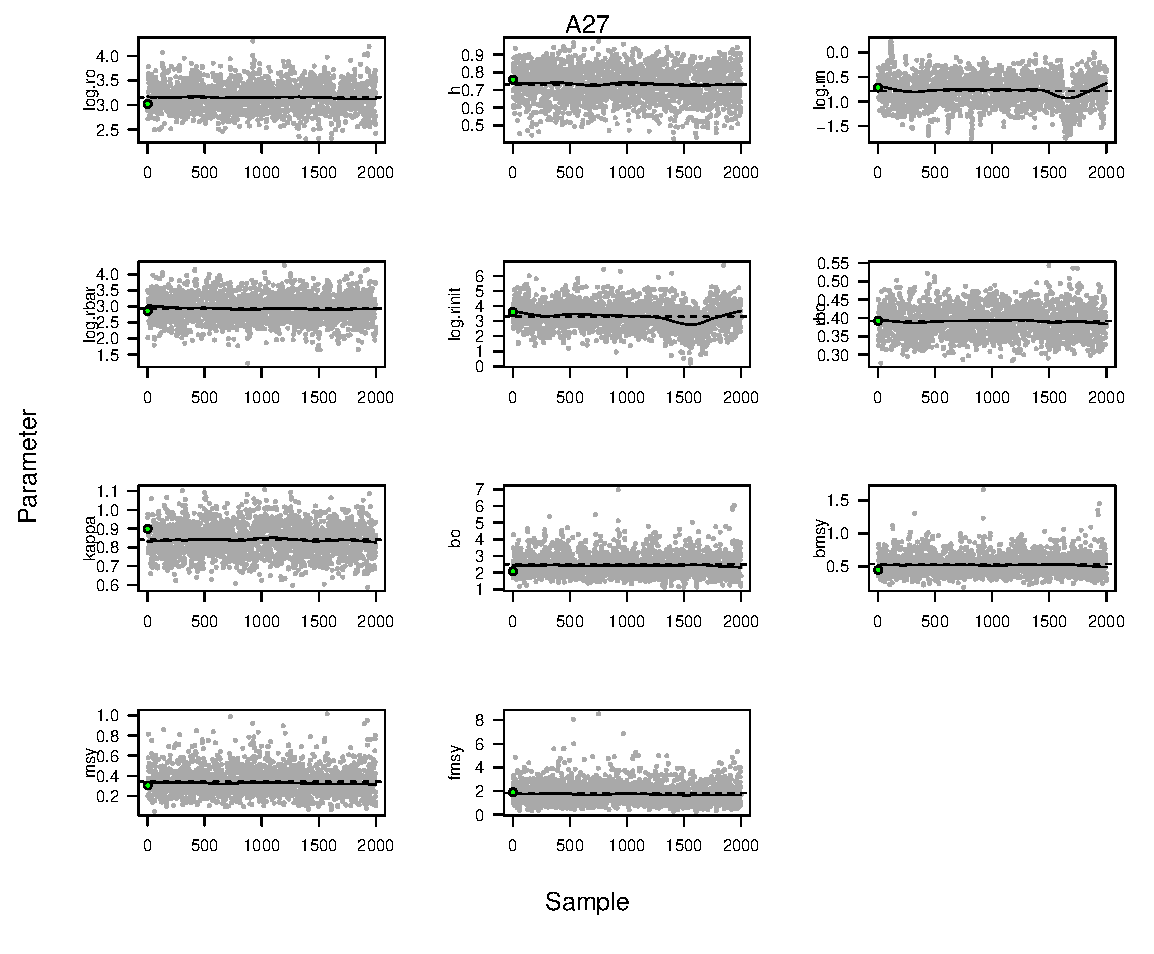
\includegraphics[width=0.75\textwidth]{../FIGS/MinorAreas/iscam_fig_traceplots_A27.pdf}}\\
	\caption{A systematic sample of 2000 points from a chain of length 1,000,000 from the joint posterior distribution for areas 2W and area 27. }\label{Results:Minor:mcmcTrace}
\end{figure}

 \begin{figure}[!tbp]
	% Requires \usepackage{graphicx}
	\centering
	\fbox{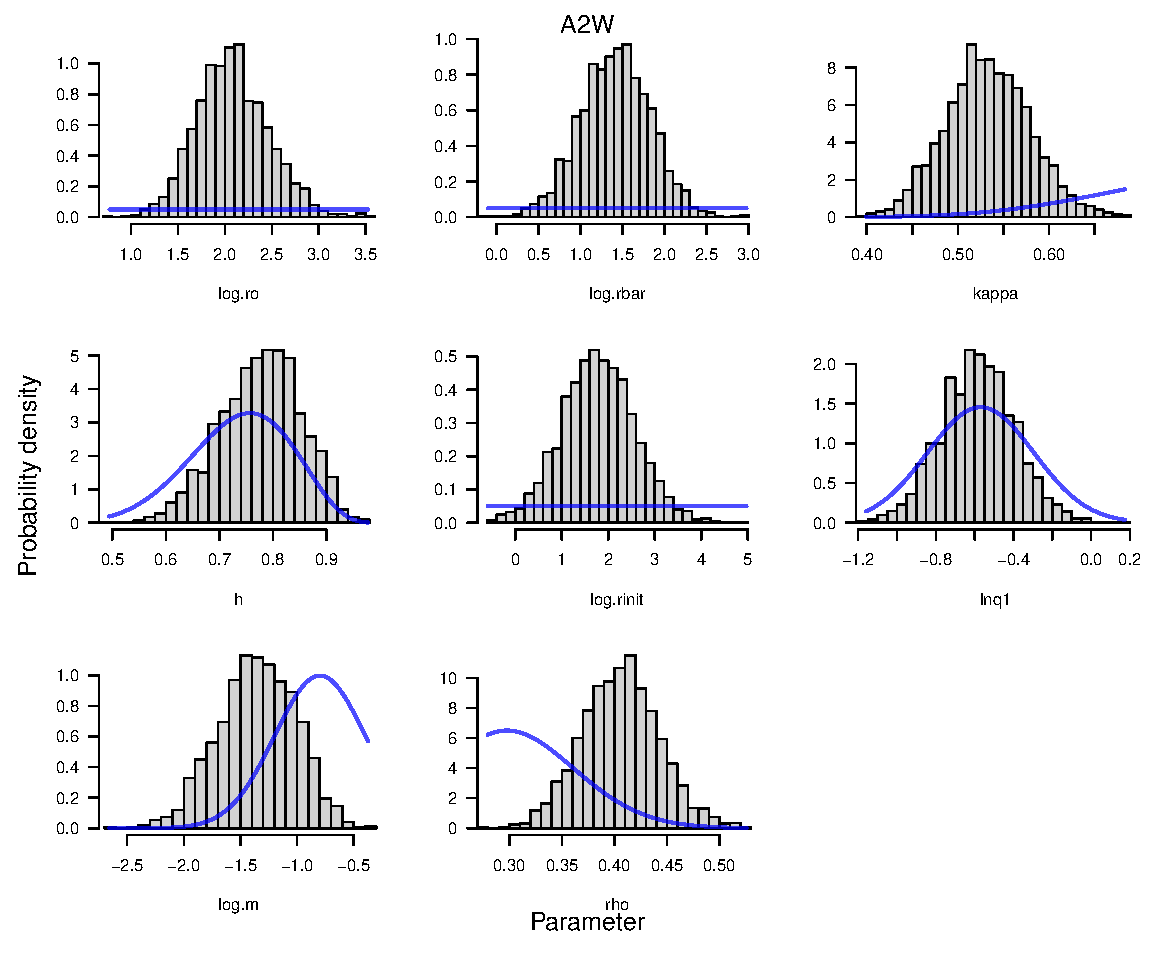
\includegraphics[width=0.75\textwidth]{../FIGS/MinorAreas/iscam_fig_marginals_A2W.pdf}}\\
	\fbox{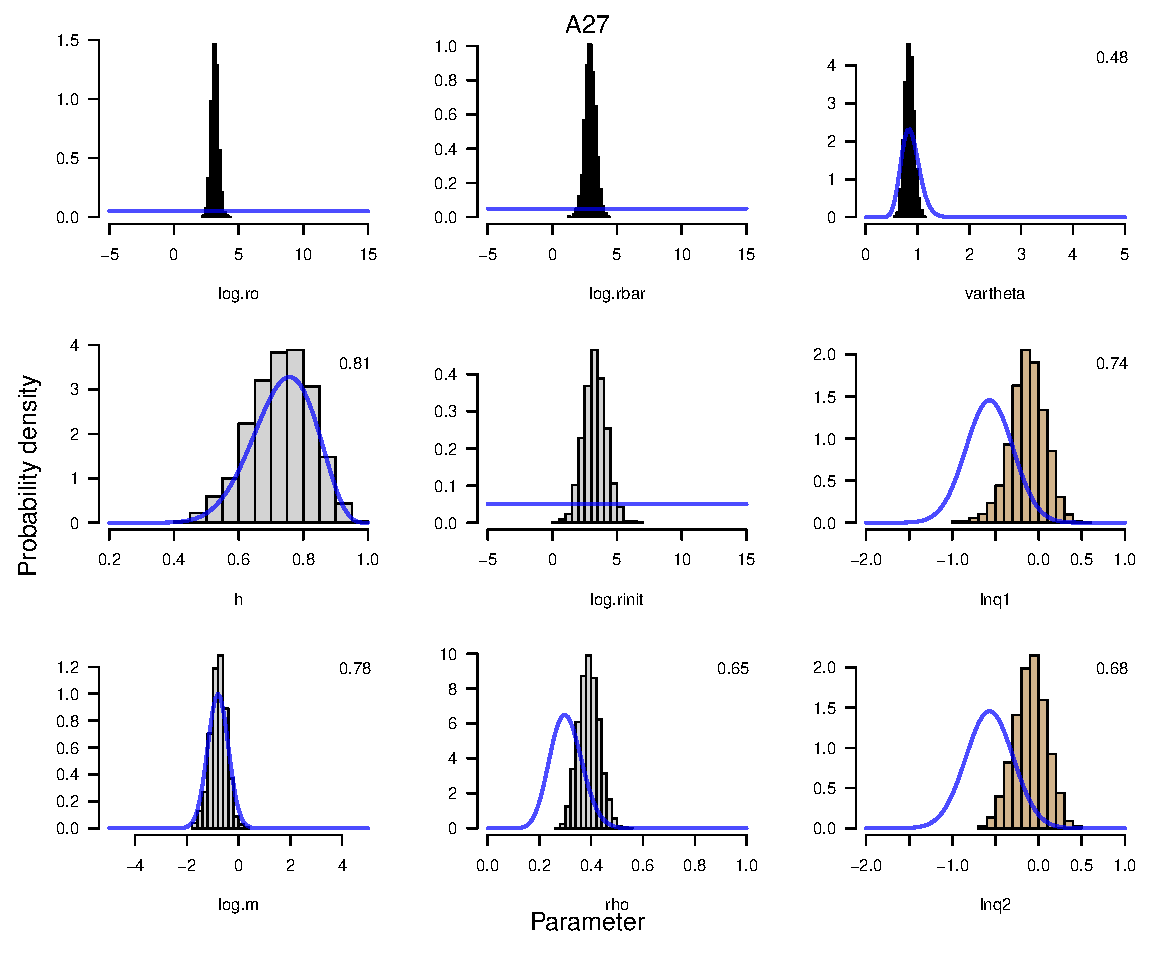
\includegraphics[width=0.75\textwidth]{../FIGS/MinorAreas/iscam_fig_marginals_A27.pdf}}\\
	\caption{Marginal distributions (bars) and priors (lines) for the leading parameters based on a systematic sample of 2000 points from a chain of length 1,000,000 from the joint posterior distribution for areas 2W and area 27.  Note the x-axis range corresponds to the lower and upper bounds of each model parameter, and the number in the top right corner is the ratio of posterior standard deviation to prior standard deviation (a ratio close to one implies no information in the data to estimate the parameter).}\label{Results:Minor:mcmcMarginals}
\end{figure}

\subsection{Catch advice}
Catch advice for the minor areas differs from that of the major areas in that there are not cuttoffs for these two areas and the reference exploitation rate is reduced from 20\% to 10\%.  The same decision table format is provided with catch advice based on poor, average, and good recruitment. Catch advice for the two minor areas is summarized in Table \ref{TableCatchAdviceMinorAreas}.


% latex.default(xTable, file = fn, rowname = NULL, longtable = FALSE,      landscape = FALSE, cgroup = cgrp, n.cgroup = ncgrp, caption = cap,      label = "TableCatchAdvice", na.blank = TRUE, vbar = FALSE,      size = "small") 
%
\begin{table}[!tbp]
 \small
 \caption{Estimated spawning stock biomass,  age-4+ biomass and pre-fishery
			biomass for poor average and good recruitment,  cutoffs,  and 
			available harvest based on median values from the joint posterior distribution for the two minor areas.  All units are reported in tonnes.\label{TableCatchAdvice}} 
 \begin{center}
 \begin{tabular}{lllclllclclll}\hline\hline
\multicolumn{3}{c}{\bfseries }&
\multicolumn{1}{c}{\bfseries }&
\multicolumn{3}{c}{\bfseries Pre-fishery forecast biomass}&
\multicolumn{1}{c}{\bfseries }&
\multicolumn{1}{c}{\bfseries }&
\multicolumn{1}{c}{\bfseries }&
\multicolumn{3}{c}{\bfseries Available harvest}
\tabularnewline \cline{1-13}
\multicolumn{1}{c}{Stock}&\multicolumn{1}{c}{SSB}&\multicolumn{1}{c}{4+ Biomass}&\multicolumn{1}{c}{}&\multicolumn{1}{c}{Poor}&\multicolumn{1}{c}{Average}&\multicolumn{1}{c}{Good}&\multicolumn{1}{c}{}&\multicolumn{1}{c}{Cutoff}&\multicolumn{1}{c}{}&\multicolumn{1}{c}{Poor}&\multicolumn{1}{c}{Average}&\multicolumn{1}{c}{Good}\tabularnewline
\hline
HG&15,202&10,080&&12,917&16,623&26,056&&     0&& 1,292& 1,662& 2,606\tabularnewline
PRD&14,859&10,272&&12,132&14,262&20,908&&     0&& 1,213& 1,426& 2,091\tabularnewline
CC& 7,213& 2,631&& 4,801& 7,044&12,470&&     0&&   480&   704& 1,247\tabularnewline
SOG&58,691&30,882&&47,169&59,423&76,324&&     0&& 4,717& 5,942& 7,632\tabularnewline
WCVI& 5,187& 1,691&& 5,745& 9,593&16,057&&     0&&   575&   959& 1,606\tabularnewline
\hline
\end{tabular}

\end{center}

\end{table}

















